\documentclass{article}
% Set target color model to RGB
\usepackage[inner=2.0cm,outer=2.0cm,top=2.0cm,bottom=2.0cm]{geometry}
\usepackage{setspace}
\usepackage[rgb]{xcolor}
\usepackage{verbatim}
\usepackage{subcaption}
\usepackage{amsgen,amsmath,amstext,amsbsy,amsopn,tikz,amssymb,tkz-linknodes}
\usepackage{fancyhdr}
\usepackage[colorlinks=true, urlcolor=blue,  linkcolor=blue, citecolor=blue]{hyperref}
\usepackage[colorinlistoftodos]{todonotes}
\usepackage{rotating}
\graphicspath{{./images/}}
\hypersetup{%
pdfauthor={Rashmi Jadhav},%
pdftitle={Homework},%
pdfkeywords={Tikz,latex,bootstrap,uncertaintes},%
pdfcreator={PDFLaTeX},%
pdfproducer={PDFLaTeX},%
}
\usepackage{booktabs}
\newcommand{\ra}[1]{\renewcommand{\arraystretch}{#1}}

\newtheorem{thm}{Theorem}[section]
\newtheorem{prop}[thm]{Proposition}
\newtheorem{lem}[thm]{Lemma}
\newtheorem{cor}[thm]{Corollary}
\newtheorem{defn}[thm]{Definition}
\newtheorem{rem}[thm]{Remark}
\numberwithin{equation}{section}

\newcommand{\homework}[6]{
   \pagestyle{myheadings}
   \thispagestyle{plain}
   \newpage
   \setcounter{page}{1}
   \noindent
   \begin{center}
   \framebox{
      \vbox{
    \hbox to 6.9251969in { {\bf CS 519:~Applied Machine Learning \hfill {\small (#2)}} }
       \vspace{4mm}
       \hbox to 6.9251969in { {\Large \hfill #1  \hfill} }
       \vspace{4mm}
       \hbox to 6.9251969in { {\it Instructor: {\rm #3} \hfill Name: {\rm #5}, Student ID: {\rm #6}} }
       %\hbox to 6.28in { {\it TA: #4  \hfill #6}}
      \vspace{1.5mm}}
   }
   \end{center}
   \markboth{#5 -- #1}{#5 -- #1}
   \vspace*{4mm}
}

\newcommand{\problem}[1]{~\\\fbox{\textbf{#1}}\hfill \newline}
\newcommand{\subproblem}[1]{~\newline\textbf{#1.}}
\newcommand{\D}{\mathcal{D}}
\newcommand{\Hy}{\mathcal{H}}
\newcommand{\VS}{\textrm{VS}}
\newcommand{\solution}{~\newline\textbf{\textit{(Solution)}} }

\newcommand{\bbF}{\mathbb{F}}
\newcommand{\bbX}{\mathbb{X}}
\newcommand{\bI}{\mathbf{I}}
\newcommand{\bX}{\mathbf{X}}
\newcommand{\bY}{\mathbf{Y}}
\newcommand{\bepsilon}{\boldsymbol{\epsilon}}
\newcommand{\balpha}{\boldsymbol{\alpha}}
\newcommand{\bbeta}{\boldsymbol{\beta}}
\newcommand{\0}{\mathbf{0}}


\begin{document}
\homework{Submission Homework 1}{Due: June 1st, 2020}{Prof. Liang Huang}{}{Rashmi Jadhav}{000-000-000}

\problem{0. Sentiment Classification Task and Dataset}
	\begin{enumerate}
		\item 	
			\begin{equation}
				RMSLE = \sqrt{\dfrac{1}{m} \sum_{i=1}^{m} (\log_e (h(x)^{(i)} + 1) - \log_e (y^{(i)} + 1))^2}
			\end{equation}

		\item
		\item
		\item
	\end{enumerate}

\newpage
\problem{1: Naive Perceptron Baseline}
	\begin{enumerate}
		\item 
		\item
		\item
		\item	
	\end{enumerate}


\problem{2: Average Perceptron and Vocabulary Pruning}
	\begin{enumerate}
		\item 
		\item
		\item
		\item
	\end{enumerate}

\newpage
\problem{3: Pruning the Vocabulary}	
	\begin{enumerate}
		\item Averaged Perceptron with one-count word pruning:\newline
		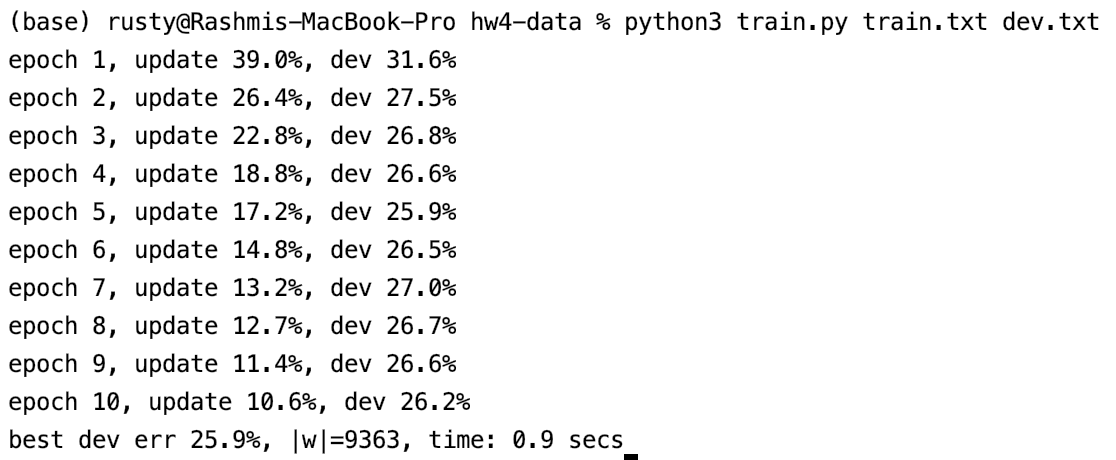
\includegraphics[width=12cm]{sample}
		\item
		\item
		\item 
	\end{enumerate}

\newpage

\problem{4: Other learning algorithms with sklearn}	
	\begin{enumerate}
		\item 
		\item
		\item
		\item
	\end{enumerate}


\problem{5: Deployment}	
	\begin{enumerate}
		\item 
		\item
		\item
		\item
	\end{enumerate}

\newpage

\problem{Debriefing}

	\begin{enumerate}
		\item 
		\item
		\item
		\item

	\end{enumerate}

\end{document} 